\chapter{Sensei}
\label{ch:sensei}

% Context
The development of the Sensei \gls{ide} plugin started in 2016, when dr. Matias Madou and Nathan Desmet founded the company Sensei Security.
I joined this company, that later would merge with \gls{scw}, as an intern a few months later.
% need and task in one
When I started my research in 2017, I set forth to discover how this tool could be used most effectively, to evaluate its concepts and features, and to help direct its design.
In this chapter, I describe the Sensei \gls{ide} plugin and discuss the lessons we learned during the implementation and testing of the tool.

\summarybox{
The first iteration of the Sensei rule editor was a \gls{gui} containing many input fields to allow fast customization of rules.
It was used by us to create hundreds of rules for customers and developer communities which frequently resulted in the need for extra features.
Some of these features are useful for improving the context awareness of Sensei and its usability, other features fell out of use.
Eventually, through the addition of these many features, the rule editor became too cluttered and unclear.

As a more flexible alternative, Nathan Desmet, principal engineer at \gls{scw}, and I designed a new formatting language based on \gls{yaml} syntax that allows rule writers to quickly and effectively create rules and quick-fixes.
The rules include several features to improve their usability and add support for libraries and for design flaws.
}

\section{Installation}

Usability of the tool starts with the installation process.
The installation of the tool should not be a hurdle but should feel like a simple customization of the developer's existing toolkit.
This is another reason why the software is distributed as an \gls{ide} plugin.

The developer's productivity benefits from their ability to customize their work environment.
More flexibility and customization allows the developer to tune their \gls{ide} to their own work habits and preferences.
It is for this purpose that IntelliJ IDEA offers an easy way to quickly install and uninstall extensions to the \gls{ide} through the Plugins menu, shown in Figure~\ref{fig:pluginsmenu}.
This menu and the JetBrains Marketplace it is connected to, allow the developer to browse and install new tools, support for new languages, additional \glspl{sdk}, extensions that help the developer learn keyboard shortcuts, or simple cosmetic changes.

\begin{figure}
  \centering
  %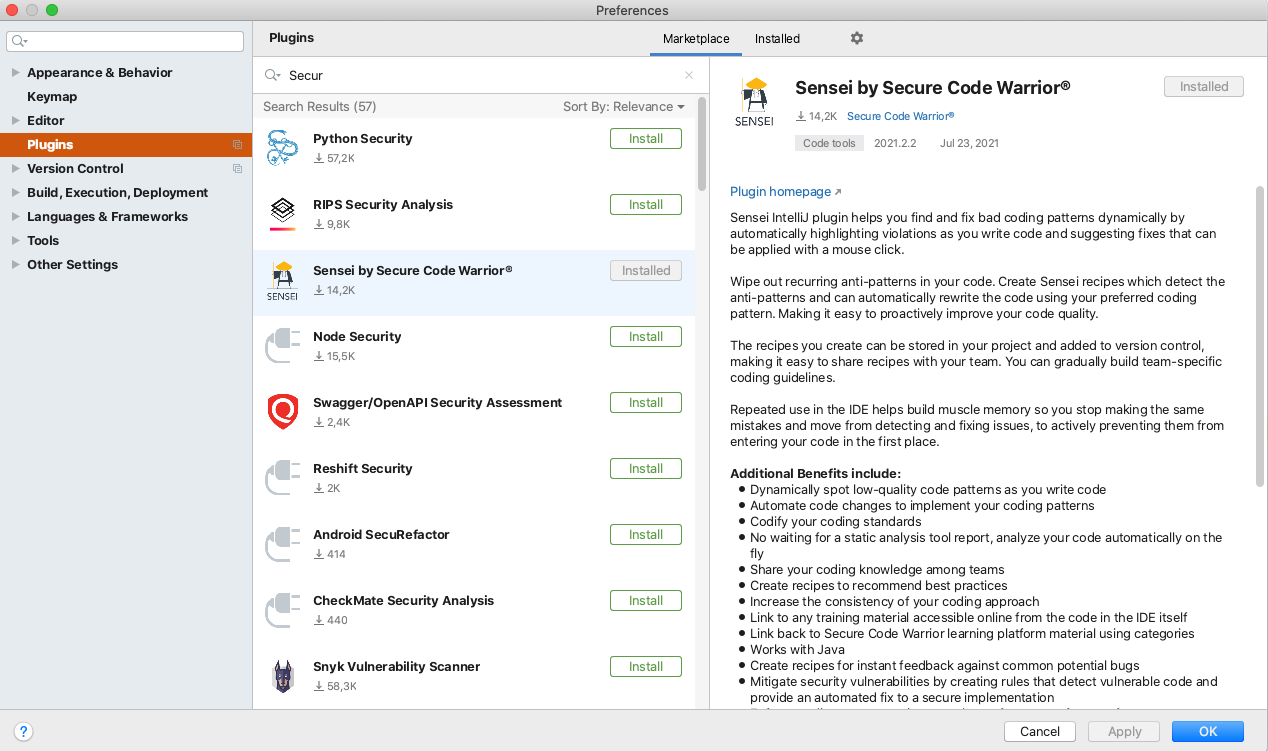
\includegraphics[width=\textwidth]{pluginsmenu.png}
  \includegraphics[width=\textwidth,page=2]{04-tools/figures/figures2.pdf}
  \caption[IntelliJ IDEA Plugins menu]{The Plugins menu in the IntelliJ IDEA allows developers to browse and easily install and uninstall extensions to their IDE.}
  \label{fig:pluginsmenu} 
\end{figure}

Sensei is available in the JetBrains Marketplace and can be installed through this Plugins menu.
Customized versions of Sensei can also be installed through this menu.
Such customized versions might be useful to disable certain features, or to automatically include certain rule sets.
To install customized versions, the Plugins menu needs to be configured to use additional plugin repositories, as shown in Figure~\ref{fig:pluginrepos}.
In this menu the developer needs to add a \gls{url} to locate the Sensei version that should be installed.
The customized version will then show up in the list of plugins in the regular menu.
This installation process is used in an experiment as described in Section~\ref{sec:experiment}.

\begin{figure}
  \centering
  %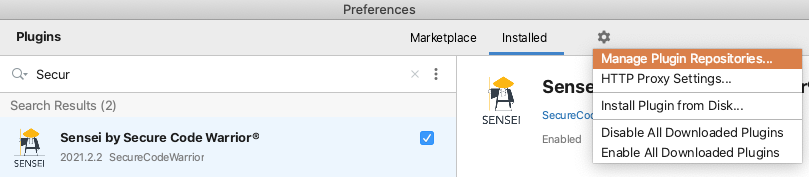
\includegraphics[width=\textwidth]{pluginrepos.png}
  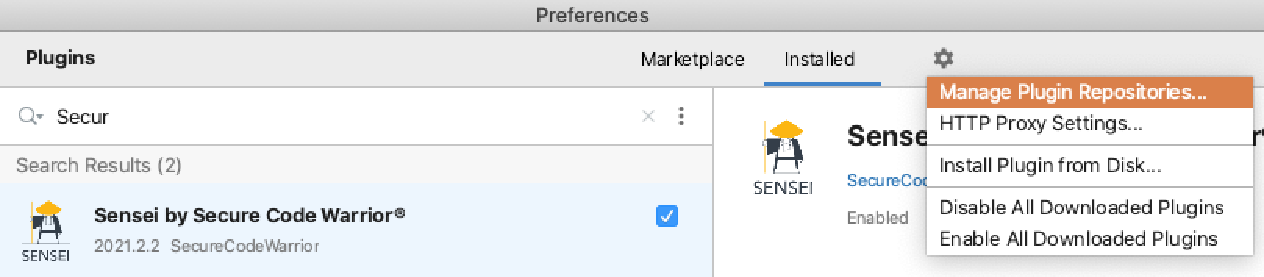
\includegraphics[width=\textwidth,page=1]{04-tools/figures/figures2.pdf}
  \caption[Adding plugin repositories to the Plugins menu]{The Plugins menu can be configured to add additional repositories of plugins, this allows us to install custom versions of the Sensei plugin that should not be distributed publicly.}
  \label{fig:pluginrepos} 
\end{figure}
\section{Recipes}

The \gls{api}-level rules that are enforced by Sensei are called recipes.
This name is chosen to emphasize the difference between Sensei and existing, traditional security tools, which often use rules to scan for vulnerabilities.
Recipes are also commonly used in the \gls{devops} movement, for example by the popular automation tool Chef~\footnote{\url{https://www.chef.io/}}.

\subsection{Creating recipes}
Customization and distribution of the recipes is a crucial feature for any successful tool supporting the paved path methodology.
If the recipes are easy to customize, Sensei can be more easily tuned to provide highly relevant and applicable feedback to the developer.
This customization should be scalable and hence not be a service provided by engineers or experts at \gls{scw}.
It should allow developers and security experts to effortlessly share project-specific or team-specific guidelines among each other.
For this reason, the recipe creation process should be easy and fast, and at the same time versatile. 

Our first approach allowed users to create new recipes through predefined recipe models.
A \gls{gui} was used to let the recipe-writer fill in a number of variables for this model.
A simple example of such a model is  the ``Replace method call model”.
Figure~\ref{fig:recipeedit2} shows a recipe being created to replace the \texttt{addCookie} method with a safe alternative from the \gls{owasp} \gls{esapi}, an open-source, web application security control library designed to make secure development easier~\cite{ESAPI}; the organization also provides some commonly used security guidelines.
The recipe-writer has to fill in some specifics about the method they want to be marked by Sensei, such as the package, class, and method names.
Then they can write one or more quick-fixes.
To create quick-fix, they have to write a quick-fix description and they have to define the code fragment that will be used to replace the original.
For the replacement code, they can reuse arguments, method names, and more from the original code by means of a template language.
In the field ``Rewrite to", the example quick-fix reuses the first argument of the original method call by using the template \texttt{arguments.0}. 

\begin{figure}
  \centering
  %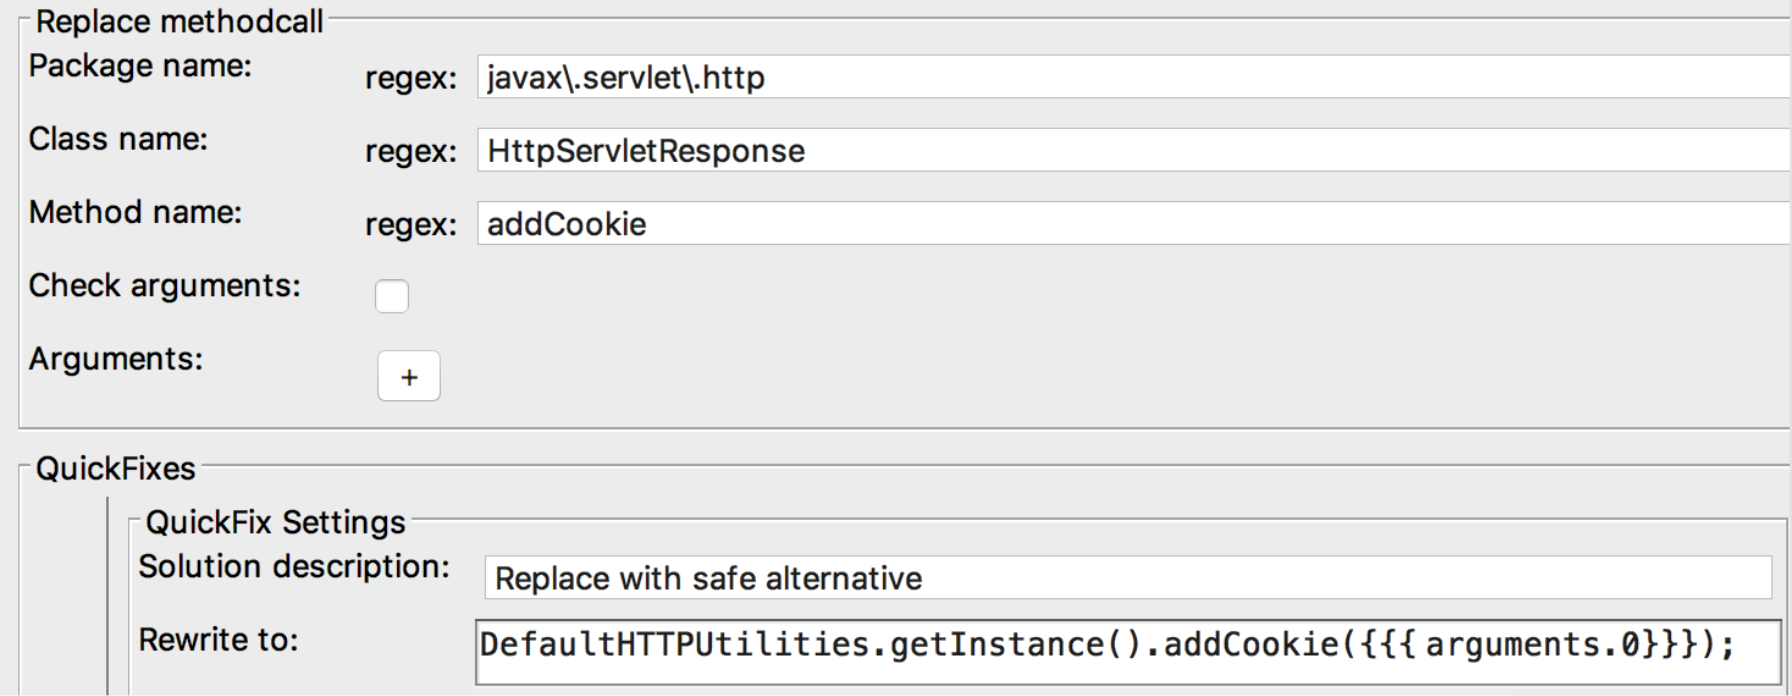
\includegraphics[width=\textwidth]{ruleedit2.png}
  \includegraphics[width=\textwidth,page=7]{04-tools/figures/figures2.pdf}
  \caption[Old model-based recipe editor]{The old recipe editor used a \gls{gui}. It required the recipe-writer to fill in a number of input fields to specify the behaviour of the recipe.}
  \label{fig:recipeedit2} 
\end{figure}

However, for more complex models the number of input fields grew rapidly to accommodate a plethora of corner cases, and so did the number of models for multiple scenarios.
As of now the old recipe editor has over 40 different models.
With this many models, it becomes overwhelming for recipe-writers that have to select a model to enforce their desired coding guideline.
The described model-based recipe creation process is not flexible and intuitive enough, so in the next iteration Nathan Desmet and I designed a new approach.

In this approach we split up the recipe in two parts: A trigger to identify the violation, plus an optional quick-fix to correct the vulnerability consistently according to company best practices.
Triggers are now specified by way of \gls{yaml}\footnote{\url{https://yaml.org/}} syntax, which provides more flexibility.
To develop this \gls{yaml} syntax, all existing Sensei rules were analyzed and grouped based on which elements in the code are incorrect and which transformations are required to fix them.
The resulting taxonomy of 10 bad code patterns is included in Appendix~\ref{app:patterns}.

Since this approach requires recipe-writers to learn the new syntax, we have provided some tools to assist them, in the form of a \gls{gui} that can be used to build the desired recipe from scratch.
In addition, the recipe editor is now more context-aware.
The recipe-writer can open a recipe creation wizard by pressing a key combination in the text editor in the \gls{ide} and selecting ``create new recipe".
This opens a context-aware menu depending on the position of the caret.
For example, if the caret was on a method call, the menu contains an option to create a new recipe that searches for similar method calls, as shown in Figure~\ref{fig:newrecipemethodcall}.

\begin{figure}[t]
  \centering
  %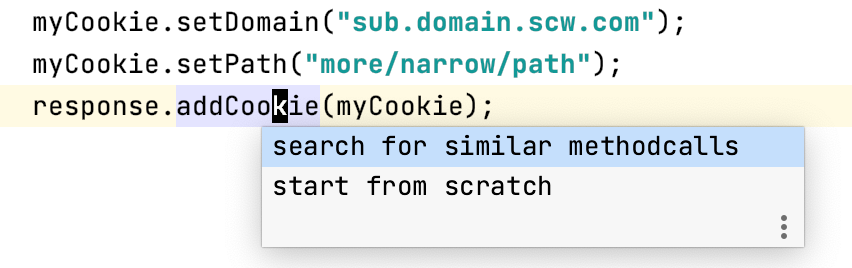
\includegraphics[width=0.8\textwidth]{rulewizard2.png}
  \includegraphics[width=0.8\textwidth,page=11]{04-tools/figures/figures2.pdf}
  \caption[Context-aware recipe creation menu]{The recipe creation menu is context aware, its options will change based on the caret position.}
  \label{fig:newrecipemethodcall} 
\end{figure}

When this context-aware option is chosen, the recipe creation wizard is opened and a recipe is automatically suggested from the available context.
To search for a methodcall, the information that can be pre-filled from context is the type and the name of the methodcall, as well as the number of arguments and each of their types.
The user can then adjust the recipe to reach the desired results through the \gls{yaml} code or the provided \gls{gui}.
This window also provides a preview panel, as shown in Figure~\ref{fig:recipewizard1}.
In this panel, the code file from which the recipe wizard was opened is shown, and the effects of the recipe being created are visualised, which allows for easy customization.

\begin{sidewaysfigure}
  \centering
  %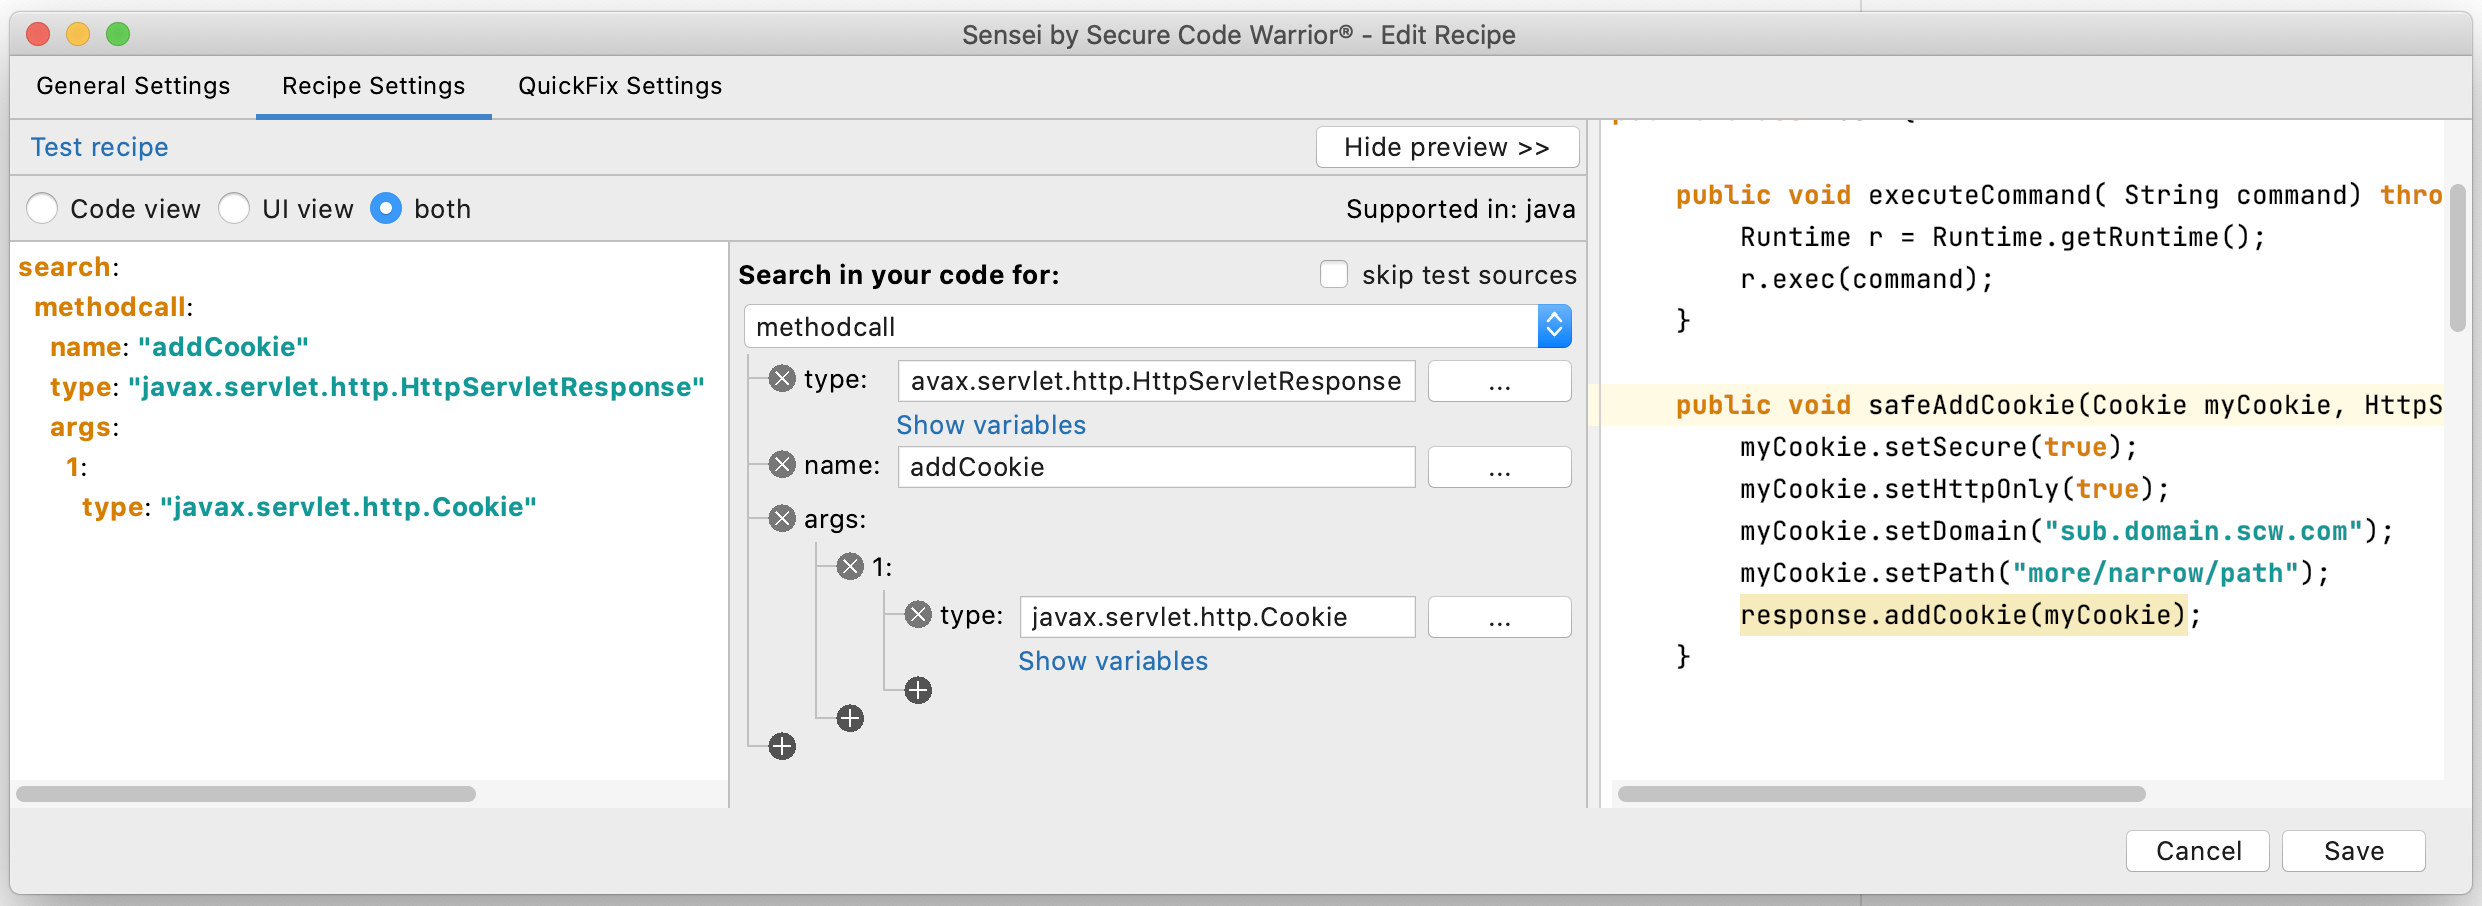
\includegraphics[width=\textwidth]{rulewizard1.png}
  \includegraphics[width=\textwidth,page=10]{04-tools/figures/figures2.pdf}
  \caption[Recipe created from context]{A recipe created through the ``search for similar methodcalls" option in the context-aware recipe creation menu will generate a \gls{yaml}-based recipe with details from the context of the caret position.}
  \label{fig:recipewizard1} 
\end{sidewaysfigure}

After creating a trigger, it is possible to create an optional quick-fix.
Here, the recipe-writer has to fill in the quick-fix description and the replacement code.
For the replacement code, they can make use of the same template language as in the first approach to reuse parts of the original code.
Below the input field, an overview is provided of the available parts of the original code, as shown in Figure~\ref{fig:createfix}.
Double clicking one of these options, adds its template to the fix.
The quick-fix creation window also offers a live preview in the lower right corner that highlights the changes that would be made to the original code (shown in the lower left corner) if the quick-fix is applied.

\begin{figure}
  \centering
  %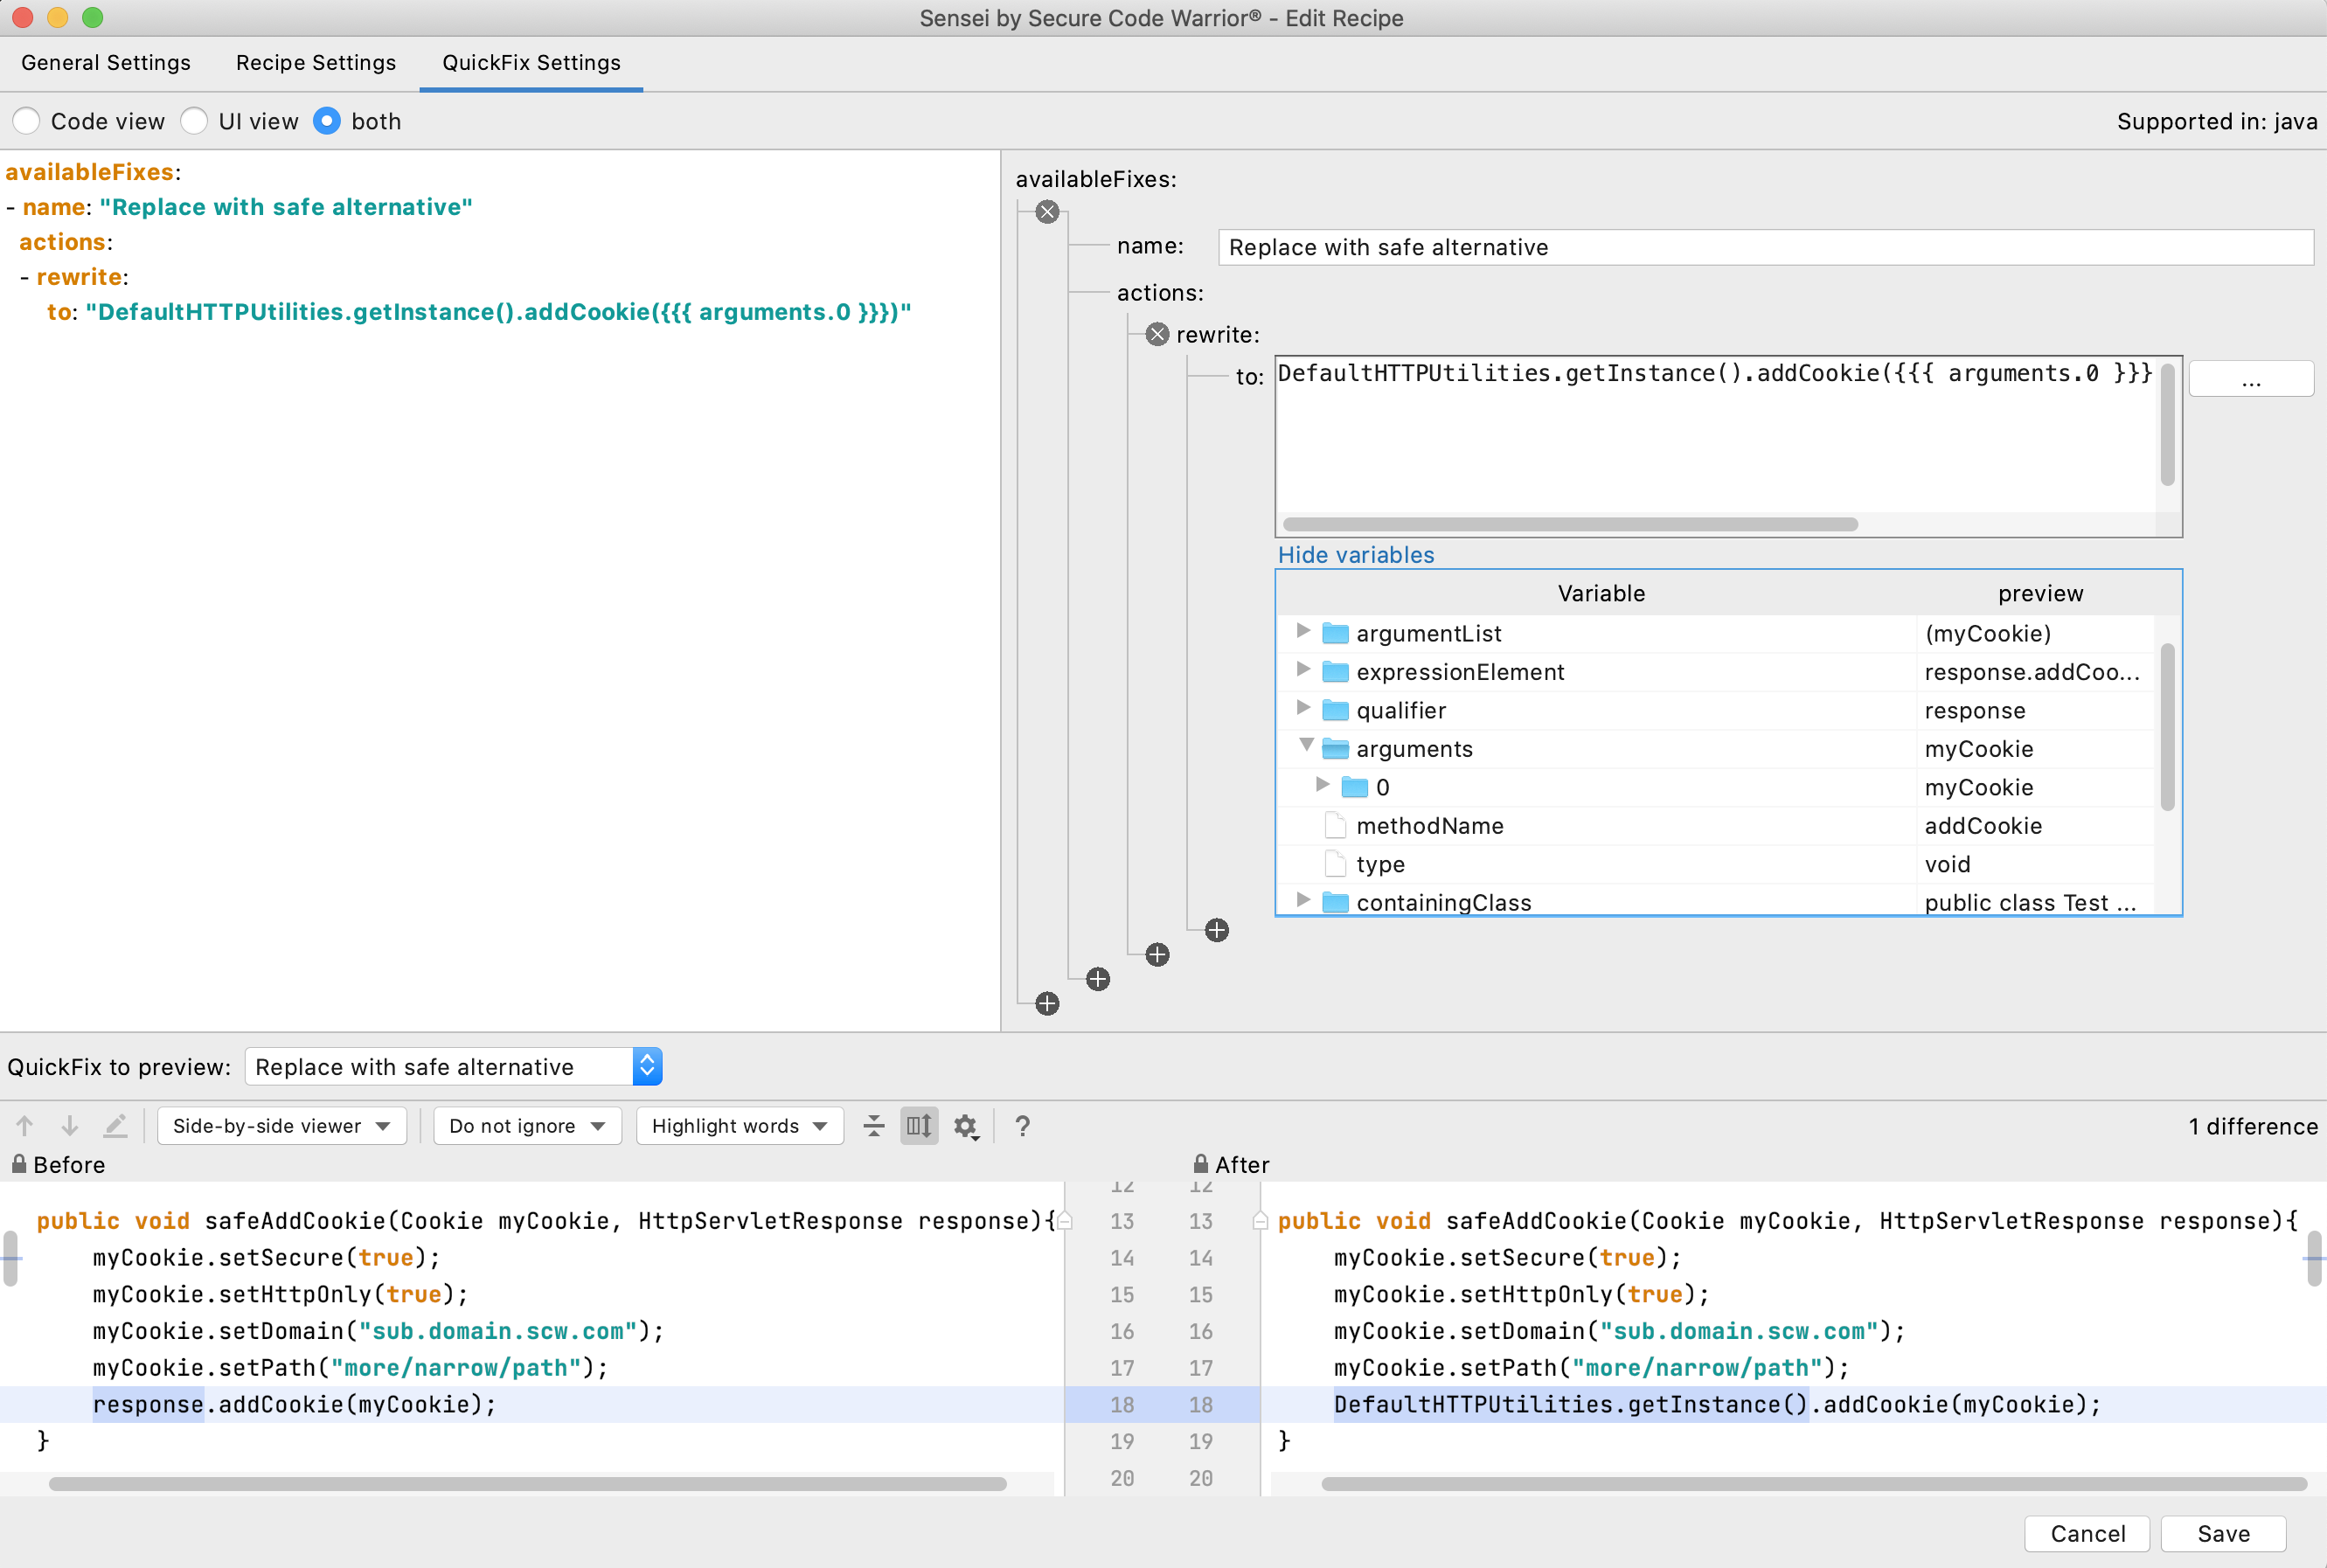
\includegraphics[width=\textwidth]{createfix.png}
  \includegraphics[width=\textwidth,page=5]{04-tools/figures/figures1.pdf}
  \caption[Fix creation window]{The fix creation window allows the recipe-writer to reuse parts of the original code.}
  \label{fig:createfix} 
\end{figure}

Finally, besides the trigger and the fix, there are also a number of general settings for the recipe that can be configured, as shown in Figure~\ref{fig:generalsettings}.
Some examples are the name, descriptions, the category of a related vulnerability, overriding recipes, and scopes.
All of these features are related to the usability of the developer and will be discussed in the following sections.

\begin{figure}
  \centering
  %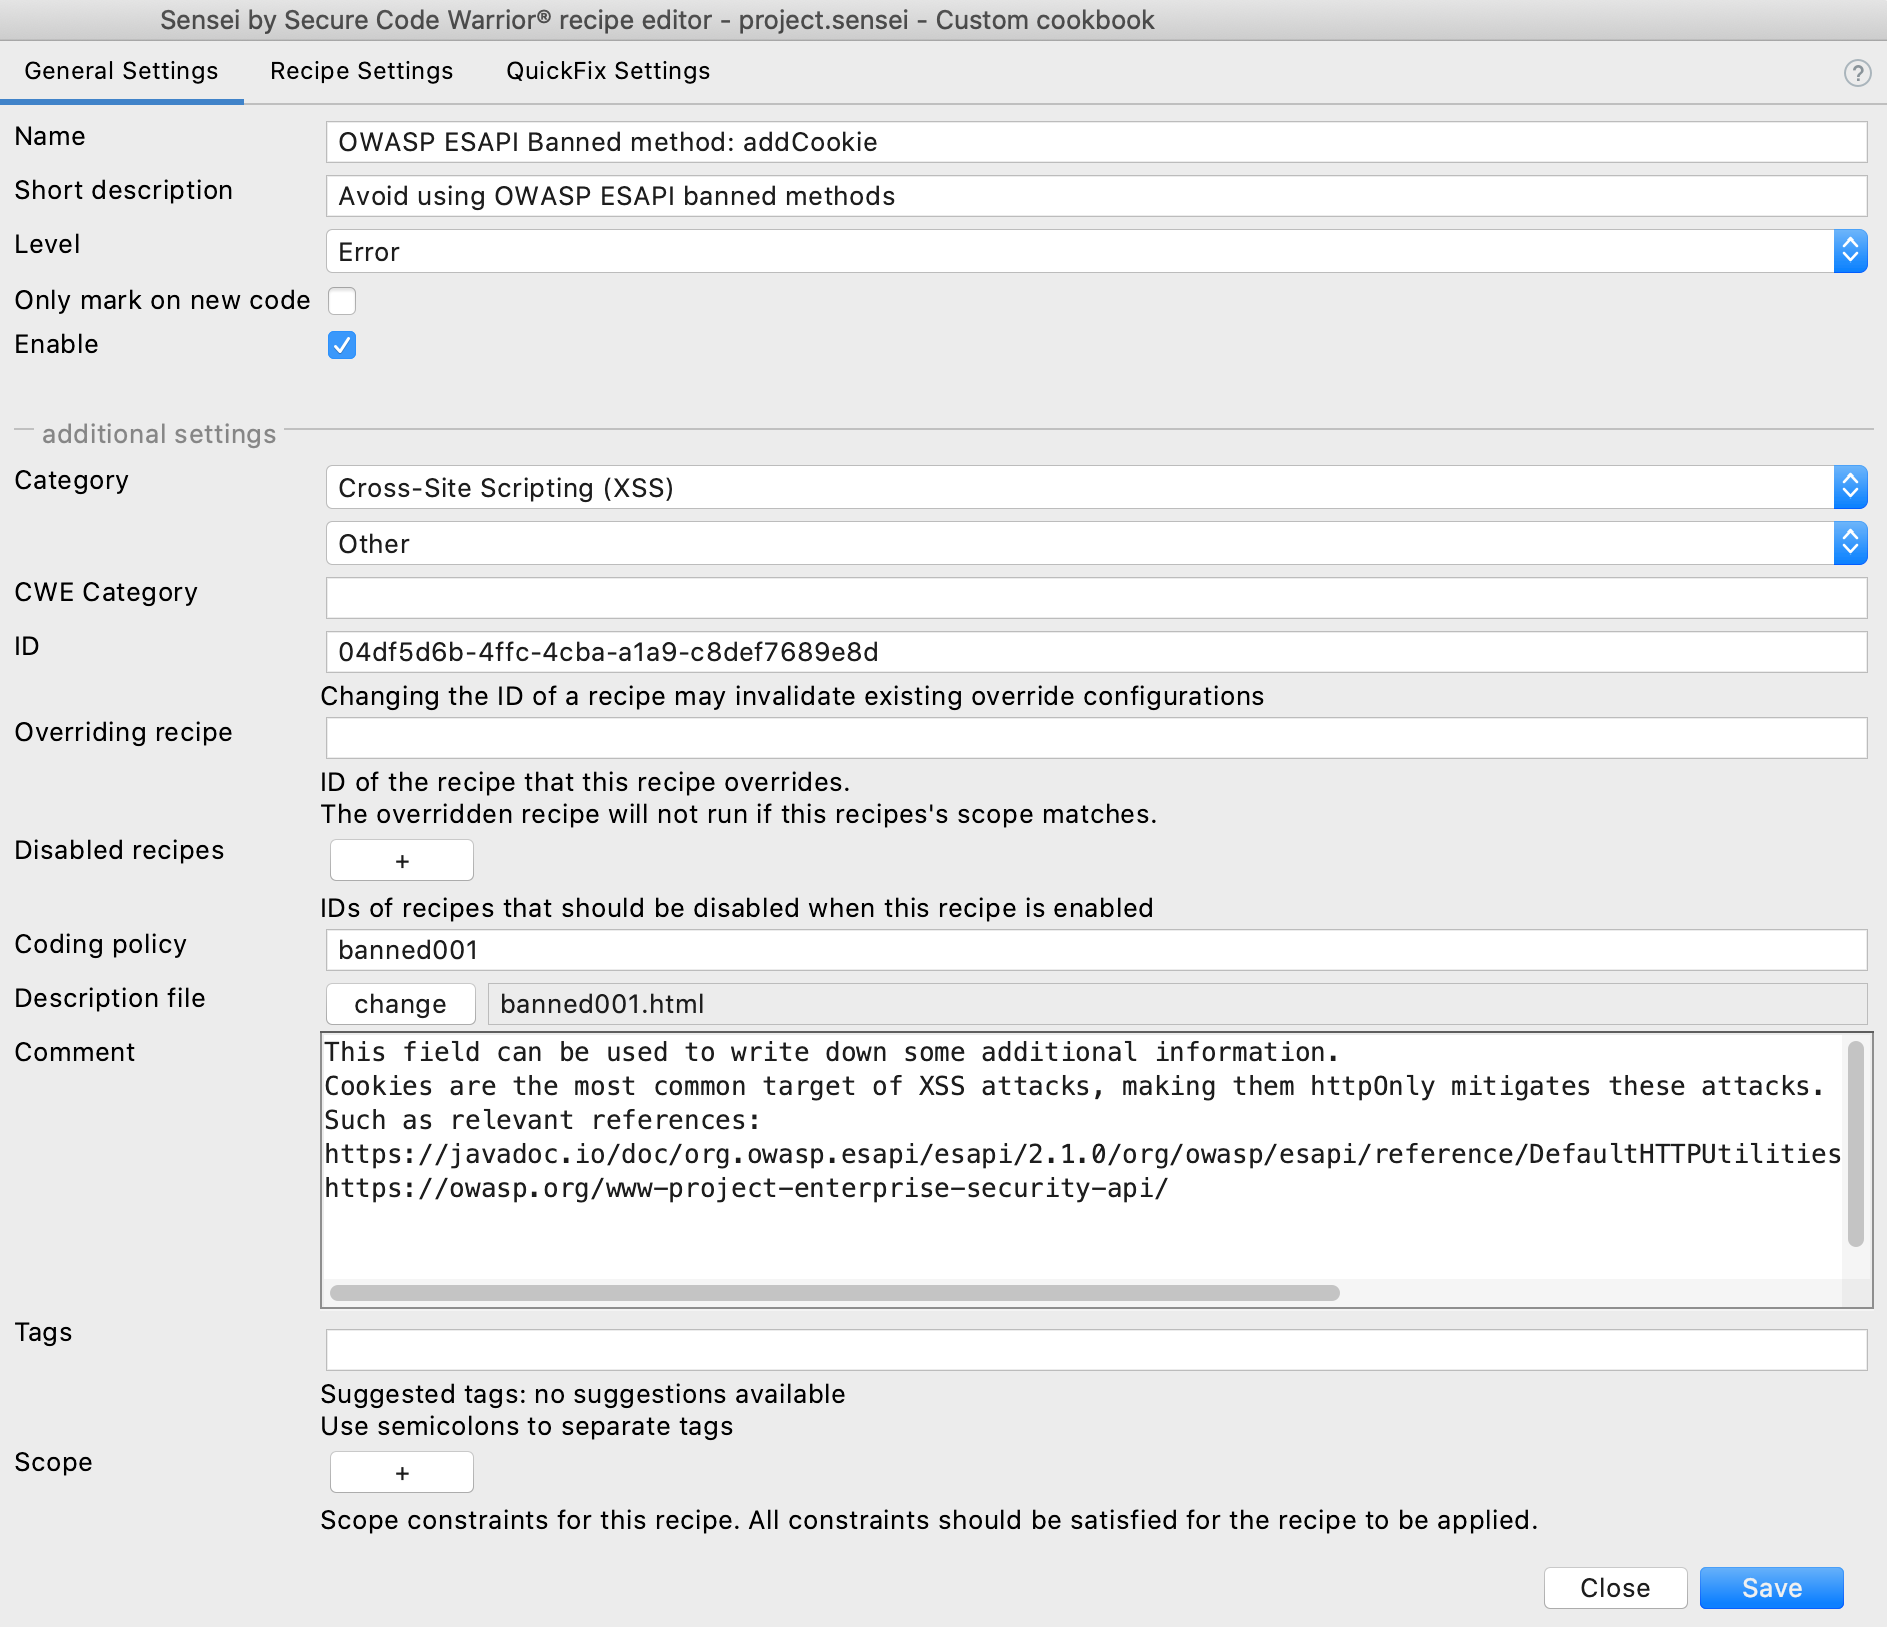
\includegraphics[width=\textwidth]{rulegeneral.png}
  \includegraphics[width=\textwidth,page=8]{04-tools/figures/figures2.pdf}
  \caption[General recipe settings]{Some additional settings are available in the recipe editor mostly related to usability of the developer.}
  \label{fig:generalsettings} 
\end{figure}

When creating recipes in-house, we have observed that the context-aware recipe wizard has greatly sped up the recipe creation process.
In practice, creating new recipes often starts from a bad code example, either when fixing a vulnerability or while reviewing the code of a colleague.
The recipe-writer can then simply open the recipe creation wizard from this example.
The live previews also greatly improve the usability, since before they were introduced, to create a finished recipe the recipe-writer was required to go back and forth several times to test the recipe in the \gls{ide} and adjust it in the recipe editor.



\subsection{Managing recipes}
\label{sec:manager}
%\todo[inline]{could you please explain how a developer would know where to consult for recipe sets, depending on which APIs are being used in a program? Bjorn: Mijn originele vraag is nog steeds geldig: Waarom denk je hier niet explicieter op te antwoorden? De vraag is volgens mij hoe developers de sets kunnen consulteren, hoe ze weten welke sets voor hen toepasbaar zijn. De vraag van de reviewer was niet hoe de regels tot stand komen.}
In the paved path methodology, guidelines can be put in place at the start of the project.
If not, at the very least, relevant guidelines should be created each time a new feature is going to be developed.
Together with those guidelines, Sensei recipes should be created as well.
The recipes, however, can also be used by the developers themselves, as a way to share knowledge.
When they develop new \glspl{api}, additionally to documentation, developers can also add Sensei recipes to the project that help their colleagues use these \glspl{api} as intended.

We also recommend to make Sensei recipes part of the remediation process when problems are found by security testing or reported through bug bounty programs.
It should be part of the process to create a recipe that prevents this same vulnerability from occurring in the future.
Currently, it is often the case that security experts run the security scans.
When problems are found, these experts guide the developers by providing them with informal, broadly applicable guidelines and checklists.
These instructions sometimes use security jargon that might not be clear to all developers, and even if they are understood, that does not guarantee the developer will be able to apply them in practice.
In the paved path methodology, security experts and developers should work together to create \gls{api}-level guidelines instead.
As part of this process, to communicate these guidelines to the rest of the team, Sensei recipes can be created as well.

For existing projects, we recommend companies to start with no recipes and use existing data on the security of their project as a starting point.
This could be the report of a penetration test, or results of vulnerability scans.
While resolving these issues in the code, developers and security experts can start building the first recipes.
Some clients of \gls{scw} have been hesitant to start with an empty security tool and, despite our recommendations to customize recipes for each project, still wish to receive starting recipes.
For this reason we have created small open-source sets of unopinionated recipes that can be used in all projects\footnote{\url{https://securecodewarrior.github.io/public-cookbooks/}}.
These recipes aid in correctly using the standard libraries of certain popular frameworks (e.g., Java 
\gls{ee}, Android \gls{sdk}, \gls{aws} \gls{sdk}).
This set can be used as inspiration and to get both security experts and developers accustomed to the tool, but usually it does not flag many issues.

Considering the different sources of recipes, developers can have recipes imposed by management and/or by the security team, as well as recipes distributed among the developers per team or project.
On top, there is the open-source recipes that can be used as a starting point when first using the tool.
To make the management of recipes easier, we group recipes into cookbooks.
Instead of distributing recipes one-by-one, this allows for grouping and distributing related recipes more easily. 

In order to manage these cookbooks in the \gls{ide}, a cookbook manager is provided, as shown in Figure~\ref{fig:cookbookmanager}.
Each cookbook is specified by a name and a location.
The developer can enable or disable any cookbook as well as edit recipes in some cookbooks.

\begin{figure}
  \centering
  %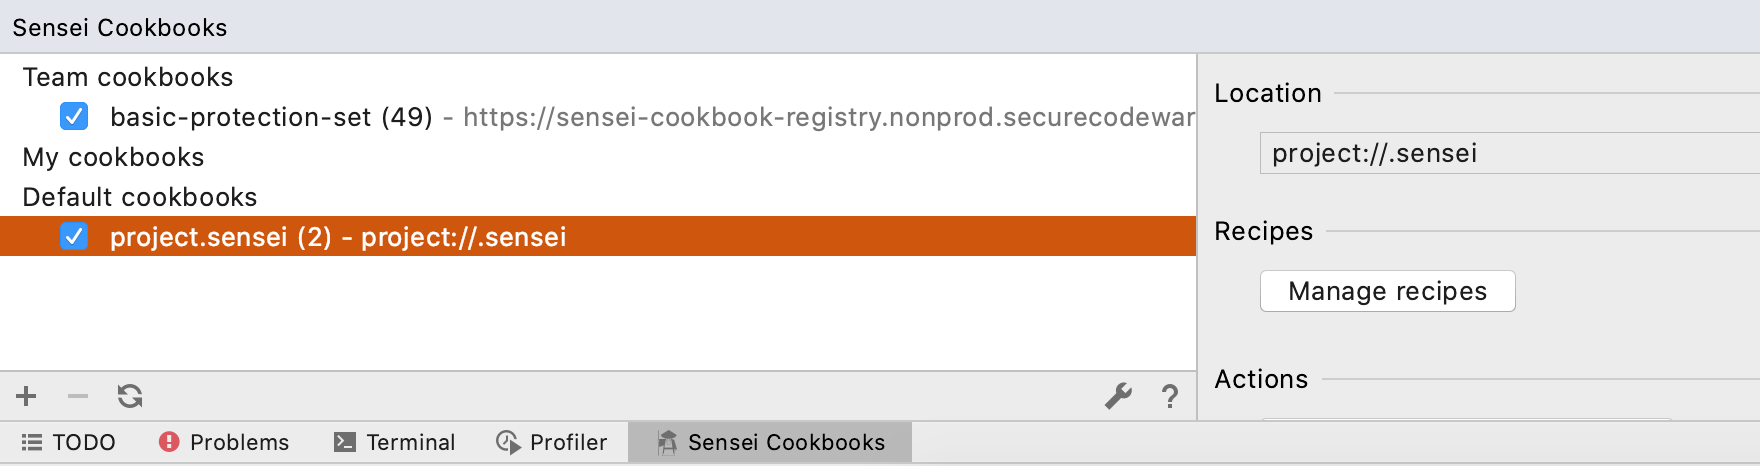
\includegraphics[width=\textwidth]{cookbookmanager.png}
  \includegraphics[width=\textwidth,page=3]{04-tools/figures/figures1.pdf}
  \caption[Cookbook manager]{The cookbook manager in this screenshot contains one remote team cookbook as well as one default cookbook stored in the project structure.}
  \label{fig:cookbookmanager} 
\end{figure}

Cookbooks can be stored locally or remotely.
Remote cookbooks are called team cookbooks and can be loaded from a github project (e.g., \texttt{git@gitserver:cookbooks|master|recipes}) or another remote server location (e.g., \texttt{https://remote.com/recipes.zip}).
Remote cookbooks are only recommended to distribute generally applicable cookbooks, since remote recipes are not editable by the developers and are instead read-only.
Any updates to the remote cookbooks are automatically pushed to all the developers.
Locally stored cookbooks are editable and can be specified by a local path (e.g., \texttt{/Users/dev/recipes}) for personal cookbooks or a path starting from the project root (by default \texttt{project://.sensei}) for default cookbooks for a project.
Local cookbooks are editable which means they can also be enabled on a recipe-by-recipe basis.
It is advised to store project specific recipes as part of the project.
This way, the recipes are always available, up-to-date with the code, and following the same flow as regular code (e.g., branch, review, merge).
When recipes follow the same flow as the code, new \glspl{api} and the recipes needed to use them properly can be added to the project and reviewed as a whole. 

The paved path methodology encourages customization of the recipes at project level.
Previous research and experience have shown that customization at at this level is the most successful.
This provides the needed flexibility to tailor the enforced coding guidelines to the code, but also ensures that the team has a joint approach to how the code for a project should be developed~\cite{sadowski2015tricorder}.
Individually customized recipes might lead to disagreements, while company-wide recipes might be too general to be easily applied.

It is possible for a recipe to be configured to disable other recipes, as shown in the general settings in Figure~\ref{fig:generalsettings}.
This feature can be used to improve remote, read-only recipes.
It is possible that such a recipe is not fully applicable to the project, e.g., because it requires too many manual adaptations.
It is then possible to create a replacement recipe that can be distributed to one team or project and disables the original recipe when it is active.
To facilitate this, an option in the quick-fix menu is added to copy remote recipes to a local cookbook, as shown in Figure~\ref{fig:copyrecipe}.
This option can easily be hidden in the settings.
The clone recipe window, shown in Figure~\ref{fig:clonewindow}, provides an option to automatically disable the original recipe it is copied from.
When a remote recipe is disabled or replaced, the author of this recipe should be notified.
It is possible that it is a generally applicable improvement and the recipe can be updated accordingly for other teams or projects that use it in a remote cookbook.
An additional quick-fix option will be added in the future to disable a recipe.

\begin{figure}
  \centering
  %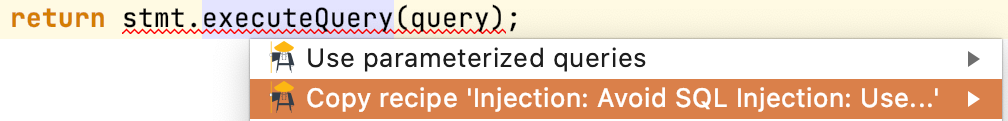
\includegraphics[width=\textwidth]{copyrecipe.png}
  \includegraphics[width=0.9\textwidth,page=4]{04-tools/figures/figures1.pdf}
  \caption[Copy recipe option in the quick-fix menu]{For remote recipes, the quick-fix menu offers a ``Copy recipe" option.}
  \label{fig:copyrecipe} 
\end{figure}

\begin{figure}
  \centering
  %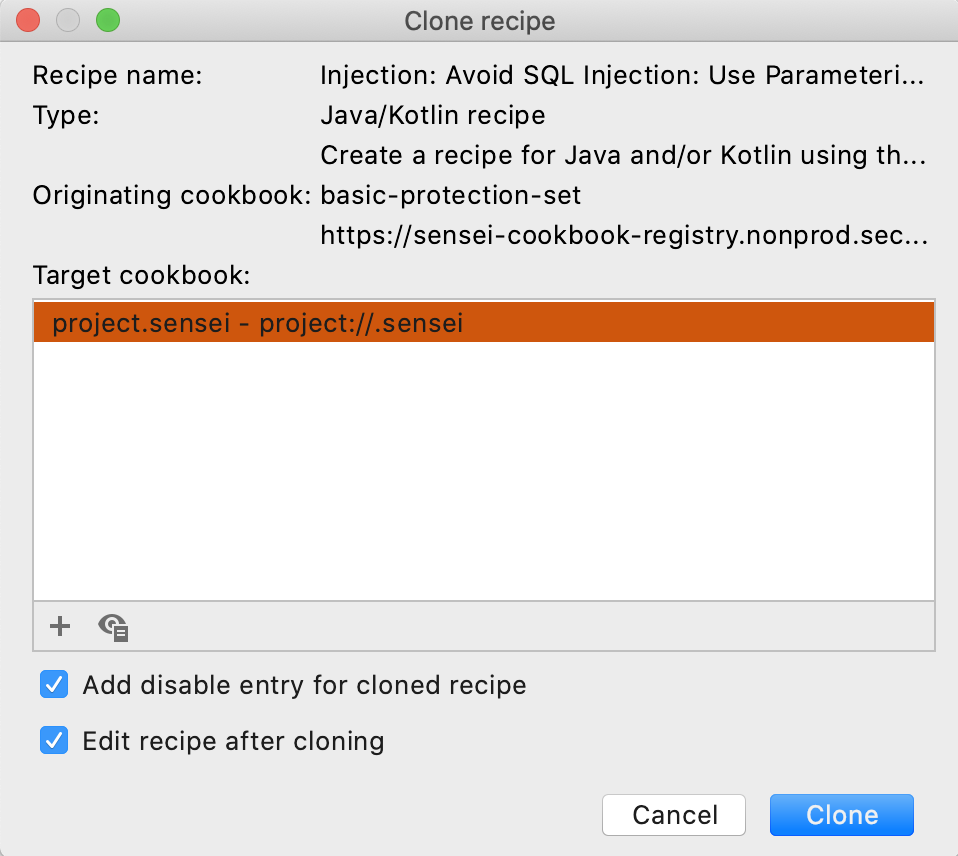
\includegraphics[width=0.75\textwidth]{clonerecipe.png}
  \includegraphics[width=0.75\textwidth,page=2]{04-tools/figures/figures1.pdf}
  \caption[Clone recipe window]{The clone recipe window allows the recipe-writer to configure the new recipe to disable the recipe it is copied from.}
  \label{fig:clonewindow} 
\end{figure}

The discussed features to disable recipes have been designed to improve the usability of the tool for developers.
They are in line with the philosophy that developers' productivity benefits from their ability to customize their development environment to their preferences, and to give them a significant amount of freedom in that regard.
In that philosophy, it is preferable to have developers disable some recipes rather then uninstalling or neglecting the tool completely.
Importantly, this does not necessarily result in guideline violations slipping below the radar, since security and management can still have these recipes, as well as complimentary tools, enabled in later phases of the \gls{sdlc}.

\subsection{Verifying recipes}
To inspect the code against a number of recipes, our tool reuses the \gls{ide} syntax checking features.
When a developer writes new code, the \gls{ide} rebuilds the \gls{ast} and computes the changes compared to the previous version.
A limited \gls{ast} of the changes, containing the necessary symbol information, is then passed on, allowing tools to only analyze the changes.
On this \gls{ast}, a combination of specialized light-weight versions of existing analysis techniques is used such as taint analysis, data flow analysis, and control flow analysis to verify the recipes in real time.

\subsection{Explaining recipes}
\label{sec:information}
In order to mark violated guidelines, our plugin makes use of existing \gls{ide} features to flag coding mistakes.
In most \glspl{ide} the code markings by default have three levels of severity: \emph{error}, \emph{warning}, and \emph{information}.
We recommend to mark coding guideline violations as errors.
Traditional error-level markings are usually immediately addressed by the developer, while warning-level markings are more frequently ignored~\cite{whitney2018embedding}.
This is the case because error-level warnings in an \gls{ide} typically indicate a problem in the code that will result in a compilation failure.
Currently error markings by our tool still allow successful compilation of a project, but several clients have requested for the markings to result in compilation failures, equivalent to errors marked by the \gls{ide} itself.
This is not surprising, as it is in line with the default behavior of popular \glspl{ide} such as Visual Studio.
For example, when Visual Studio's C compiler compiles code that uses the insecure \texttt{sprintf} function, it throws a compilation error warning the developer that the function may be unsafe.

An example marking can be seen in Figure~\ref{fig:publicactivity}, where the opening \texttt{<activity>} tag in \gls{xml} code is marked as an error.
This marking makes the code fragment stand out and attracts the developer's attention.
In the example, the Android activity is configured as a public activity by setting the \texttt{exported} attribute to \texttt{true} but not configuring an intent filter.
In \gls{xml} code, like in this example, it is advised to only mark the opening tag, and not the entire \gls{xml} tag and its content.
This would overwhelm the developer, and it would not be clear which part of the code is lacking. 

\begin{figure}
  \centering
  %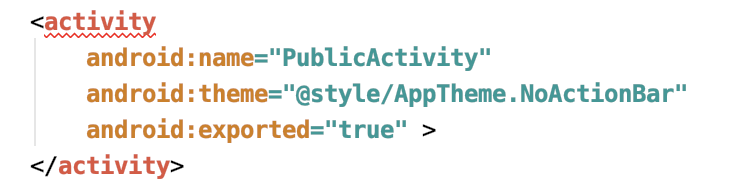
\includegraphics[width=.75\linewidth]{publicactivity.png}
  \includegraphics[width=0.75\textwidth,page=3]{04-tools/figures/figures2.pdf}
  \caption[Error marking on an XML opening tag.]{\Gls{xml} recipes can be configured to mark the opening tag only (shown in the figure), the opening tag and the closing tag, or both tags and their entire content.}
  \label{fig:publicactivity} 
\end{figure}

Permanent markings, that remind developers of security implications of their decisions, should be marked as information.
To continue on the example of private and public activities, in the code file that implements the activity, we mark the class definition at the information level.
Hovering over the marking informs the developer whether the activity is configured as public or private, and provides a direct link to detailed information about the security implications.
This marking is shown in Figure~\ref{fig:infomarking}.
Note how the markings are clearly visible and noticeable, but at the same time non-intrusive to developers already used to their \gls{ide} flagging code fragments.

\begin{figure}
  \centering
  %
\includegraphics[width=0.80\linewidth]{infomarking2.png}
  \includegraphics[width=0.8\textwidth,page=10]{04-tools/figures/figures1.pdf}
  \caption[Marking at the information error level]{The information error level marking is clearly visible but at the same time non-intrusive, as this is a permanent marking that can not be resolved.}
  \label{fig:infomarking} 
\end{figure}

The marking of code is accompanied by three descriptions.
The information in these descriptions is important to ensure the continued use of the tool~\cite{whitney2018embedding,layman2007toward}.
Developers build trust with analysis tools, and this trust is quickly lost if they do not understand the tool’s output~\cite{bessey2010few}.
The first description is the short error description, i.e., the text that appears when the developer hovers their mouse pointer over the marked code.
It should be just one line.
The purpose of this description is to attract attention, inform the developer that something should be addressed, not to explain how to address it.

We have learned through user feedback that it is most effective to attract the user's attention by starting with the “why”~\cite{RSAvideo}, the reason the code is marked and should be addressed.
In the past the short description used to indicate the possible vulnerability class, for example “Could lead to SQL injection”. 
We believed that starting with the potential consequences, makes the developers realize the severity of their mistake and encourages them to immediately address it.
However, as explained in Section~\ref{sec:communication}, security jargon should be avoided when communicating to developers.
The feedback in all of the descriptions should be targeted at developers, and hence the focus should be on the guidelines that were put in place, on the paved path.
A better short description is hence, “Violates a guideline on data retrieval”, as depicted in Figure~\ref{fig:shortdescription}.

\begin{figure}
  \centering
  %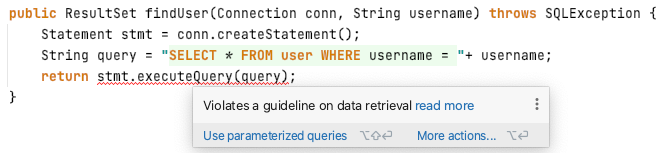
\includegraphics[width=\linewidth]{shortdescription2.png}
  \includegraphics[width=\textwidth,page=14]{04-tools/figures/figures2.pdf}
  \caption[Short description of a recipe]{The short description of a recipe is visible when hovering over a marking. It should attract the developers attention but avoid security jargon. Instead, the developer can be reminded of guidelines that are in place.}
  \label{fig:shortdescription} 
\end{figure}

Next to the short description a “read more” link is created by the \gls{ide} for the interested developer.
Upon clicking this link, a pop-up is opened to show a more elaborate \gls{html} page.
This is the second description.
Figure~\ref{fig:fulldescription} shows an example.
This description is called the full coding guideline.
The page starts with a short abstract, stating in one sentence what should be done, such as “Secure coding practices prescribe that queries need to be parameterized”.
The page's next section presents in detail what it means to use parameterized queries and gives an overview of the approved \gls{api} methods.
Small code examples are included as well, since previous research has shown examples are the fastest way for developers to understand a problem~\cite{whitney2018embedding}.
The goal of this description is after all to help developers find out quickly how to comply to the coding guideline without spending much time or effort.
This is crucial for a security tool to feel well integrated into developer workflows.
The last section of the description contains a list of possible consequences when the developer fails to address this issue.
There is no mention of vulnerabilities or exploits until this point.
Each item in the list contains a link to the \gls{scw} training platform to learn more about the vulnerabilities and how they are exploited.
This way an interested developer (with too much time on their hands?) can still easily find the necessary information to learn the details of each vulnerability and the possible attacks.
Following this training would require a context switch and would likely hurt developer productivity.
In the future the integration between the \gls{scw} training platform and the Sensei \gls{ide} plugin can be improved as described in the perspectives in Section~\ref{sec:its-integration}.

\begin{figure}
  \centering
  %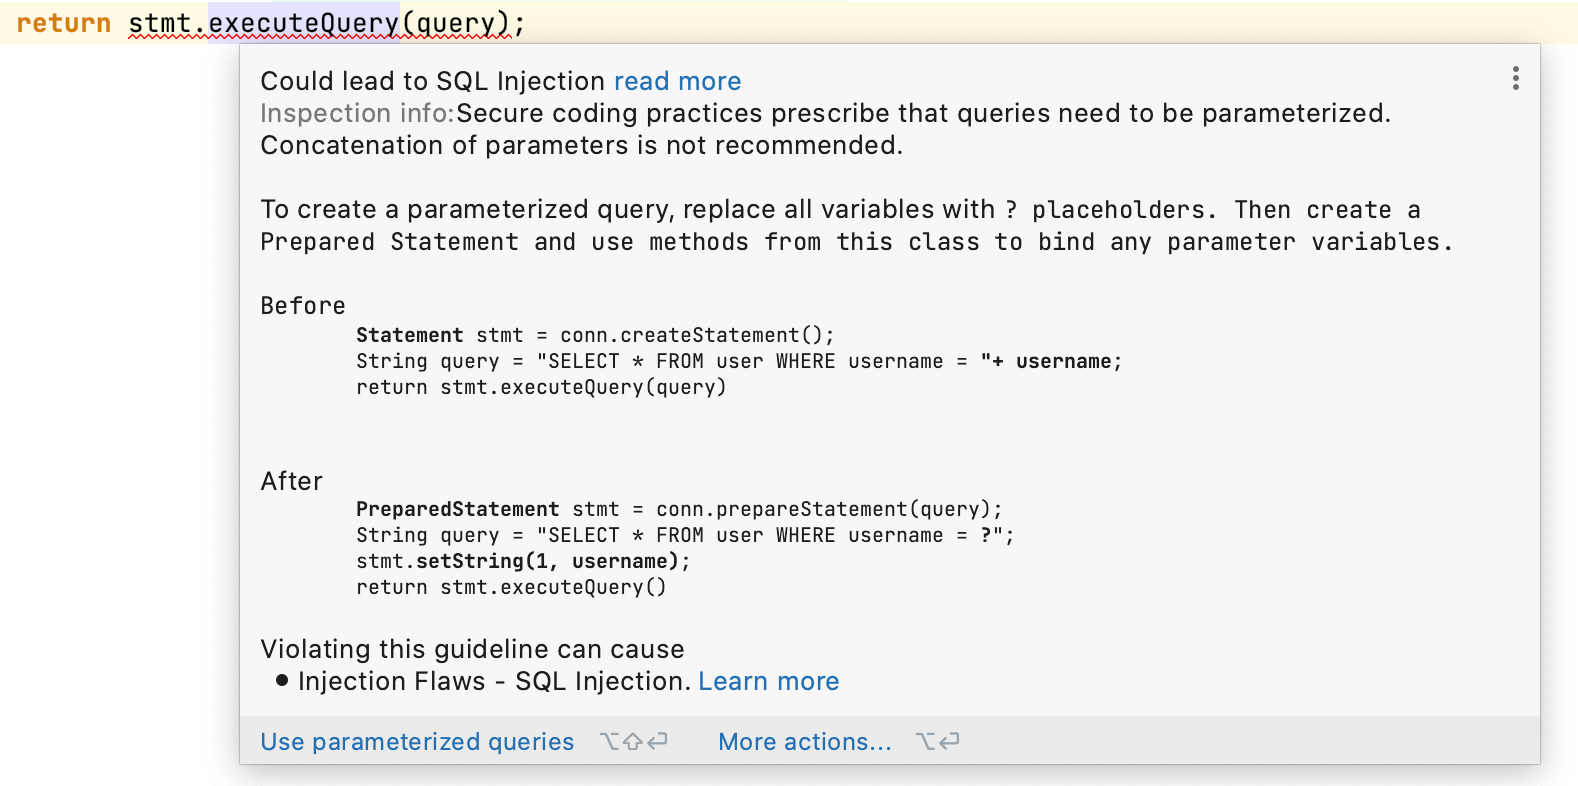
\includegraphics[width=\textwidth]{guideline.png}
  \includegraphics[width=\textwidth,page=7]{04-tools/figures/figures1.pdf}
  \caption[Example of the full coding guideline.]{The full coding guideline is a more elaborate \gls{html} page that explains the guideline in more detail and provides code examples.}
  \label{fig:fulldescription}
\end{figure}

The third description is visible to the developer when they press the \gls{ide}’s key combination to start resolving the issue.
A drop down menu appears, containing the possible quick-fixes' descriptions.
%A "copy recipe" option is available as well, and for local recipes there is also additionally an "edit recipe" option, both of these can be disabled in the Sensei settings.
IntelliJ also provides options to disable inspections locally or globally. Figure~\ref{fig:qfdescription} shows an example.
In this menu we provide a very short description of the actions that will be performed when this code transformation is chosen, such as “Use parameterized queries”.
A brief yet descriptive quick-fix description allows developers to decide quickly whether the fix is appropriate for them.
If the effects of applying the quick-fix are well understood, the developer will trust the tool and apply the fixes more often.
Sometimes the developer needs to choose between different possible solutions.
However, it is advised to keep the number of fixes as low as possible, as to not complicate the issue unnecessarily.

\begin{figure}[t]
  \centering
  %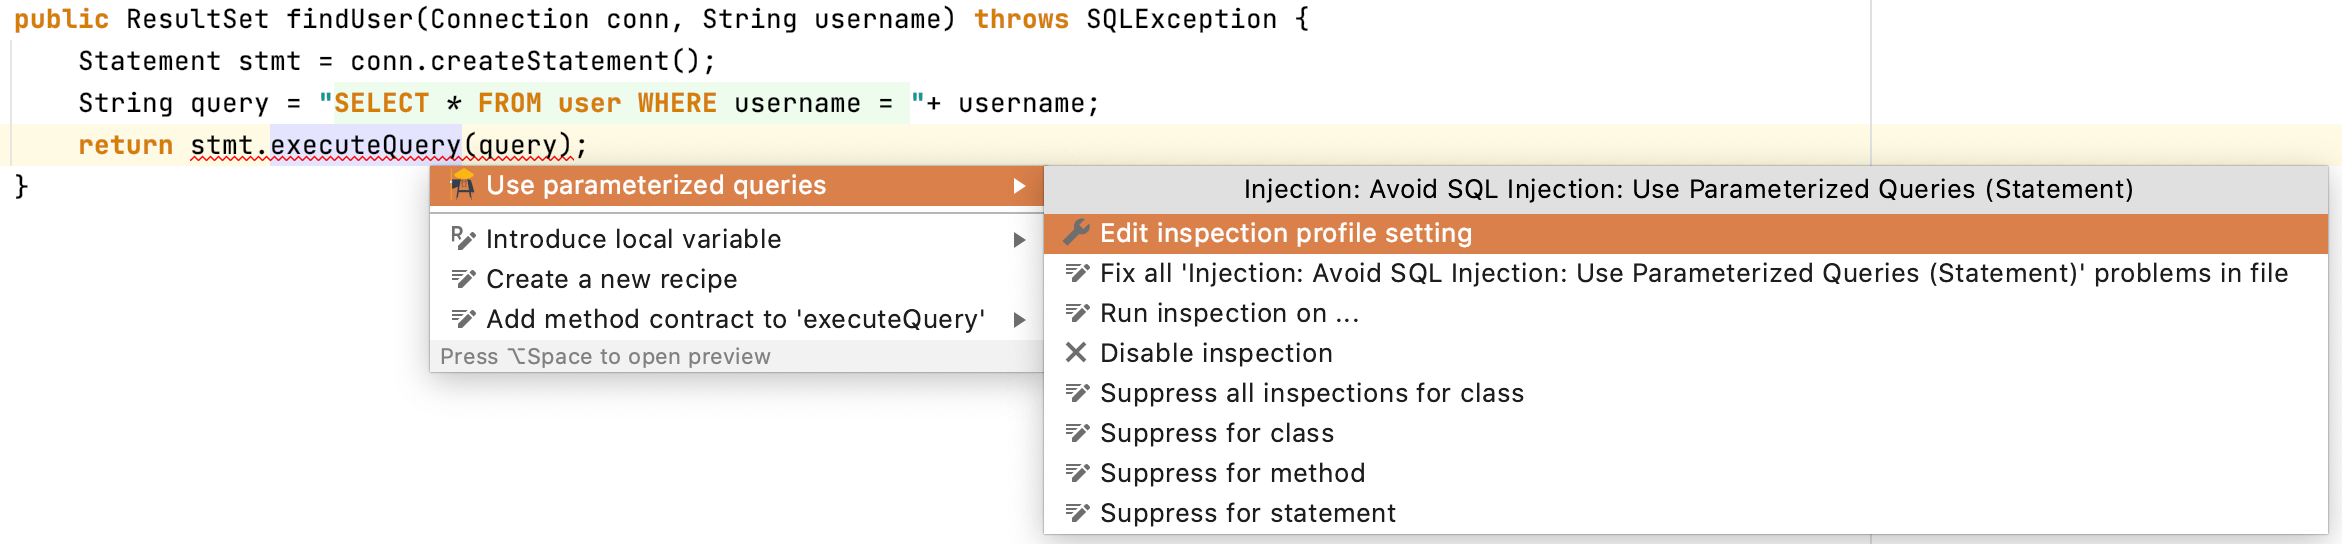
\includegraphics[width=\textwidth]{quickfixmenu.png}
  \includegraphics[width=\textwidth,page=5]{04-tools/figures/figures2.pdf}
  \caption[Example of the quick-fix description.]{The quick-fix description briefly describes the actions that will be performed when each option is chosen. IntelliJ also offers a feature to suppress markings of any inspection (Sensei or otherwise).}
  \label{fig:qfdescription} 
\end{figure}

\section{Recipe features}
\label{sec:features}

Over time, several advanced features in the recipes have been developed following user feedback.
In this section, I explain the problems they tackle and provide code examples for each one.

\subsection{Lowering effective false positives}
\label{sec:efp}
It is important to choose the right error level for the developer to pay attention to the markings, but also not to overwhelm them with markings to the point that they start to ignore them.
Since the recipes can be created by anyone in the team, they should not be too obtrusive.
To a recipe writer, a false positive is an incorrect marking of code that is not violating a coding guideline.
However, to a developer, a false positive is any code marking that they do not intend to fix and ignore instead~\cite{ayewah2007evaluating}.
A false positive from the perspective of the developer is also called an \gls{efp}~\cite{sadowski2015tricorder}.
To ensure the usability of the tool, the \gls{efp} rate should be sufficiently low~\cite{sadowski2015tricorder,johnson2013don}.

To demonstrate \glspl{efp} we take a look at \gls{os} Command injection.
One of the \glspl{api} that is banned in the \gls{owasp} \gls{esapi} guidelines is \texttt{Runtime.exec}.
This \gls{api} is used to execute \gls{os} commands in Java programs.
When user input is added to this command, \gls{os} command injection is possible and the attacker can gain access to the underlying \gls{os}.
Using this information it is possible to create a recipe that marks all uses of the \texttt{Runtime.exec} method.
While this is a good coding guideline, a security conscious developer recognizes that the method needs user input before it can lead to \gls{os} command injection.
In rare occasions an \gls{os} command might be necessary for functionality and perfectly valid and secure.
For example, launching another software product can be done securely as long as the command is hard-coded.
An example of insecure usage of the \texttt{Runtime.exec} method can be found in Listing~\ref{lst:oscommand1}, examples of secure usage in Listings~\ref{lst:oscommand2}~and~\ref{lst:oscommand3}.
The two secure examples are still violations of the above coding guideline, and they get flagged.
An experienced developer has no intent to fix them, meaning they are two cases of \glspl{efp}.
Notice how this \gls{efp} depends on the knowledge and skill of the developer, meaning that it might be beneficial to adjust the feedback of the tool for individual developers, as explained in the perspectives in Section~\ref{sec:sensei-perspectives}.
%A similar example leading to \glspl{efp} is when hard-coded \gls{sql} queries are created without using parameterized queries.
%These queries would violate a guideline enforcing parameterized queries, but they would not be insecure, not even when this function is reused from a different context in the future.

In order to keep the \gls{efp} rate sufficiently low we have introduced the concept of \emph{trusted input}.
Hard-coded input is automatically trusted, since a user can not influence it, and hence it can not lead to a vulnerability.
However, function parameters and variables from other origins are considered untrusted by default.
This is still in line with the philosophy to protect methods from future use, where we want to flag violations that can one day lead to vulnerabilities.
The requirement in recipes of untrusted input can be added to arguments, this can be done using the \gls{yaml} syntax or by using the \gls{gui} as shown in Figure~\ref{fig:recipegui}. 
The next step is to define trusted sources. This also avoids the \gls{efp} in Listing~\ref{lst:oscommand3}. The resulting recipe can be seen in Listing~\ref{lst:yamlrecipe}.

\begin{minipage}[t]{0.9\linewidth}
%\vspace{-0.4 cm}
\begin{lstlisting}[language={Java},caption={if the \texttt{command} variable contains unsanitized user input, this function is vulnerable to \gls{os} command injection.},label={lst:oscommand1},abovecaptionskip=-0.0pt,xleftmargin=15pt]
public void executeCommand(String command){
    Runtime r = Runtime.getRuntime();
    r.exec(command);
}
\end{lstlisting}
%\vspace{-0.3cm}
\begin{lstlisting}[language={Java},caption={Using a hard-coded command avoids the possibility that the variable will ever contain unsanitized user input.},label={lst:oscommand2},abovecaptionskip=-0.0pt,xleftmargin=15pt]
public void executeCommand(){
    Runtime r = Runtime.getRuntime();
    r.exec("explorer.exe");
}
\end{lstlisting}

\begin{lstlisting}[language={Java},caption={This code fragment is secure if the \texttt{getSafeCommand} method can be trusted to never return variables containing unsanitized user input.},label={lst:oscommand3},abovecaptionskip=-0.0pt,xleftmargin=15pt]
public void executeCommand(){
    Runtime r = Runtime.getRuntime();
    String command = getSafeCommand();
    r.exec(command);
}
\end{lstlisting}

\begin{lstlisting}[language={yaml},caption={This recipe trigger requires the argument of an \texttt{exec} methodcall to contain untrusted input before it will mark the methodcall. It also specifies the methodcall \texttt{getSafeCommand} as a trusted source of input.},label={lst:yamlrecipe},xleftmargin=15pt]
search:
  methodcall:
    name: "exec"
    type: "java.lang.Runtime"
    args:
      1:
        type: "java.lang.String"
        containsUntrustedInput: true
        trustedSources:
        - methodcall:
            name: "getSafeCommand"
\end{lstlisting}
\end{minipage}
%\vspace{-.3cm}

\begin{figure}[t]
  \centering
  %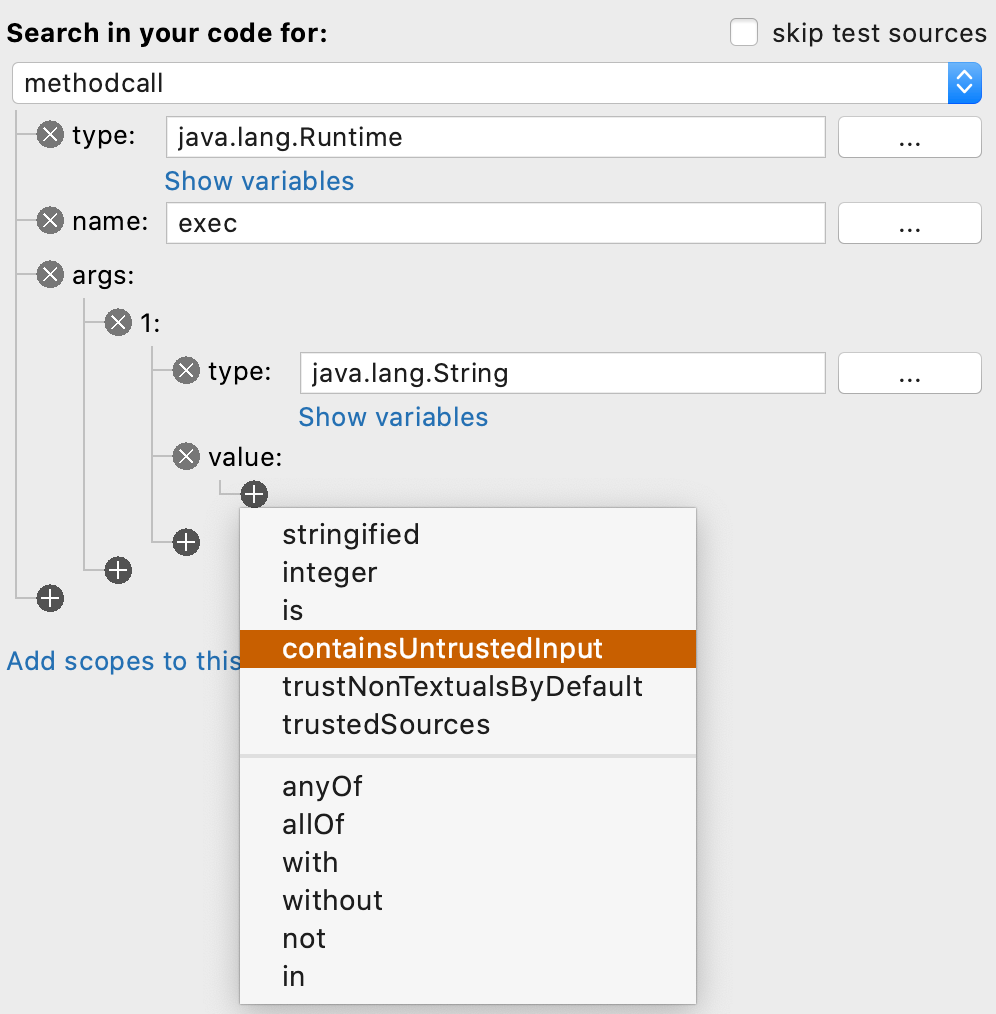
\includegraphics[width=\textwidth]{rulegui2.png}
  \includegraphics[width=\textwidth,page=9]{04-tools/figures/figures2.pdf}
  \caption[\Gls{gui} to add the requirement of untrusted input.]{It is possible to add requirements like untrusted input or an in-clause through the \gls{gui}.}
  \label{fig:recipegui}
\end{figure}

Another way to allow recipe writers to create more targeted recipes and to keep the \gls{efp} rate low, is to provide \emph{trigger scopes}.
Trigger scopes can be added by using the \texttt{in} keyword in the \gls{yaml} syntax, or by using the \gls{gui} as shown in Figure~\ref{fig:recipegui}.
The in-clause can define restraints on the context.
This makes it possible to create a recipe that prevents the usage of \texttt{Runtime.exec} except in a class with name \texttt{AppLauncher}.
Scopes like this can also help with performance, i.e., meeting the real-time checking requirement, since recipes that are out of scope can be skipped during analysis.

In the old editor, rather than \emph{trigger} scopes, \emph{recipe} scopes were a property of the entire recipe.
They were added by selecting the type of scope and filling in some fields.
By migrating these scopes to the \gls{yaml} syntax, the scoping of recipes becomes much more flexible.
The recipe scopes that can be migrated to trigger scopes are the class scope, method scope, file scope, Android context scope, and Android build property scope.
Descriptions of these scopes can be found in Appendix~\ref{app:recipe-scopes}.

There are two more recipe scopes, for which migration to trigger scopes is not useful.
The \emph{project scope} allows us to enable or disable recipes based on the name of the project.
This is useful when different cookbooks are required for each project in a company.
This scope is no longer needed since we now allow cookbooks to be stored in the project, which is a lot more convenient then adding a scope to each recipe separately.
The \emph{library scope} can be used to enable recipes based on the presence of a library.
This way we can disable a recipe if the fix uses a library that is not used in the project.
Since this scope is created for the fix of the recipe and not the trigger, it cannot be added to the \gls{yaml} syntax and remains a property of the entire recipe.
In the future it could be useful to add scopes to quick-fixes, so that a recipe can provide different fixes depending on the presence of a library.

\subsection{Support for libraries}
Often quick-fixes are small code changes, such as adding a preceding method call or changing a parameter, but sometimes they involve more elaborate pieces of code.
An example for this is adding a cookie to a \gls{http} request.
Before adding the cookie, it needs to be properly configured.
Insecure and secure code examples are shown in Listings~\ref{lst:cookie1} and~\ref{lst:cookie2}, respectively.

\begin{lstlisting}[float,language={Java},caption={This cookie is not configured before it is added to the response, as a result this code fragment is insecure.}, float,label={lst:cookie1},abovecaptionskip=-0.0pt]
Cookie myCookie = new Cookie("secure", "success");
response.addCookie(myCookie);
\end{lstlisting}

\begin{lstlisting}[language={Java},caption={Several configuration options are added to narrow the scope that the cookie can be used, and to ensure it is not sent over plaintext.}, float,label={lst:cookie2},abovecaptionskip=-0.0pt]
Cookie myCookie = new Cookie("secure", "success");
myCookie.setSecure(true);
myCookie.setHttpOnly(true);
myCookie.setDomain("sub.domain.scw.com");
myCookie.setPath("more/narrow/path");
response.addCookie(myCookie);
\end{lstlisting}

If this fix is applied at multiple locations in a project, it can result in code bloat.
It might then be better for the company to provide a method that replaces the original \texttt{addCookie} method.
In this method the cookies can be first configured properly before calling the original \texttt{addCookie} method.
Such replacement wrapper methodcall is shown in Listing~\ref{lst:cookie3}.
The new guideline for cookies is then to replace the \texttt{addCookie} method with the \texttt{safeAddCookie}, as shown in Listing~\ref{lst:cookie4}.
The creation of such a wrapper library is strongly recommended by the paved path methodology, as the resulting guidelines are very easy to understand by developers.
At the same time any security bugs are confined to the \textit{implementation} of the wrapper library, and no new bugs can be introduced by \textit{using} the wrapper library. This makes the job of the security team easier as well.

\begin{lstlisting}[language={Java},caption={A wrapper library can be created to avoid code reuse and to improve clarity of the guidelines for the developer.}, float,label={lst:cookie3},abovecaptionskip=-0.0pt] 
public void safeAddCookie(Cookie myCookie, HttpServletResponse response){
    myCookie.setSecure(true);
    myCookie.setHttpOnly(true);
    myCookie.setDomain("sub.domain.scw.com");
    myCookie.setPath("more/narrow/path");
    response.addCookie(myCookie);
}
\end{lstlisting}

\begin{lstlisting}[language={Java},caption={Migrating to the wrapper library consists of replacing the original methodcall with one from the library.},float,label={lst:cookie4},abovecaptionskip=-0.0pt]
Cookie myCookie = new Cookie("secure", "success");
safeAddCookie(myCookie, response);
\end{lstlisting}

The first example, where the cookie is configured properly, is a \emph{library usage recipe}.
This type of recipe provides guidance on using a library correctly.
The trigger of the recipe is on \glspl{api} from the library.
Code fragments are refactored without involving additional libraries, only libraries that are also used in the trigger.

The second example, where the insecure code is replaced with \gls{api} calls from a different library, is a \emph{library adoption recipe}.
Instead of providing guidance on the correct usage of the \glspl{api}, such recipes promote the adoption of a new library.
This type of recipe has a trigger in one library but their fix uses a different library.

As a proof of concept for library adoption recipes, support has been developed for the \gls{owasp} \gls{esapi} library.
Among others, the \gls{owasp} \gls{esapi} contains replacement methods for commonly used insecure \gls{jdk} methods, the so-called \gls{owasp} \gls{esapi} banned \glspl{api}\footnote{\url{https://www.owasp.org/index.php/ESAPI\_Secure\_Coding\_Guideline}}.
To support the \gls{owasp} \gls{esapi} in companies that adapt it, a recipe set was created to enforce the replacement of the banned \glspl{api} with their alternatives from the \gls{owasp} \gls{esapi}.
Feedback from these companies showed that this set of library adoption recipes was intuitive and easy to use for developers.
Importantly, it increased the speed of the library's adoption.

Library usage recipes are generally applicable to codebases because the trigger and fix of these recipes use \glspl{api} from the same library, thus ensuring that the recipes never mark any code when the fix is unavailable.
The trigger and fix for library adoption recipes depend on different libraries.
This implies that an applied quick-fix can result in the use of unavailable \glspl{api}. 

Library scopes can be used for this purpose.
When the library used in the quick-fix serves as a scope of a recipe, it will not mark any code if the library is unavailable.

\subsection{Support for detecting design flaws}
As discussed before, coding guidelines are enforced through mostly local analyses.
This allows Sensei to intervene earlier in the development process and makes it possible to perform the analyses in real time while the developer is typing.
For this reason the focus of the approach is mostly on implementation bugs.
Detecting design flaws in the application code (rather than in the \glspl{api} it relies on) is typically much harder.
Still, we have learned that various flaws can be tackled through the use of configuration files and the previously described trigger and recipe scopes.

An example of a flaw that is difficult to detect with local analyses is excessive security logging.
It is crucial to log important security events, but too much logging can make it difficult or impossible to locate certain events.
While enforcing guidelines can help with logging securely (e.g., not logging sensitive data, not logging unsanitized input, logging in proper format) it is difficult to monitor the frequency of the logging through local analyses.
Other examples are the use of transport layer security, or whether authorization is needed or not.

One scenario that, to the contrary, enables us to detect some design flaws, is when popular frameworks are used to handle security features.
For example, enforcing the use of transport layer security in an Android app is as simple as adding a line to the Android manifest about clear text traffic.
This can be seen in Listing~\ref{lst:manifest}, line 3.

\begin{lstlisting}[language={XML},caption={When the attribute \texttt{usesCleartextTraffic} is added to the Android manifest with value \texttt{false}, the Android \gls{os} will ensure that transport layer security is used for the communication with this application.},float,label={lst:manifest},abovecaptionskip=-0.5pt]
<application
     android:label="@string/app_name"
     android:usesCleartextTraffic="false">
\end{lstlisting}

Another example is the use of encryption.
It is trivial to detect if a deprecated encryption algorithm is used by means of a known \gls{api}, but it is much harder to detect the absence of encryption through local analyses.
One interesting class of mistakes that we observed was developers XOR’ing data, or encoding data, rather than encrypting it.
As a solution, a coding guideline can be created that requires functions whose name contains “encrypt” to perform encryption through some of their approved \gls{api} methods.
If such a function \emph{only} performs encoding or XOR operations, it implies that the required \gls{api} calls are missing.
In that case the tool suggests quick-fixes that insert the necessary \gls{api} calls.
These quick-fixes are only partial fixes: They inject code that invokes encryption routines on an unspecified string or byte array.
It is then still up to the developer to remove the XOR operations and fill in the correct string or array identifier.
This emphasizes again why it is beneficial to provide fixes in the \gls{ide} during development time.
When this recipe is used during the development of a new method, the developer starts by creating a function declaration.
When a function exists with ``encrypt" in the name and an empty body, this is marked, as the required \gls{api} calls are missing.
The fix then inserts the required \gls{api} calls, leading to comfortable and intuitive security help for the developer.
This recipe is a good example to demonstrate the paved path methodology.
It guides the developer along a predetermined path laid out for them to implement encryption securely.

We have also improved context-awareness to detect flaws by adding more recipe scopes.
One such example is the Android \emph{context scope}.
As explained earlier, in the Android manifest a developer can configure capabilities of components such as activities and broadcast receivers regarding their communication towards the \gls{os}.
They can listen to any other application, only to authorized applications, or only to the own application.
The Android context scope allows us to enable recipes based on the configuration of the relevant component, so that we can enforce different recipes for different levels of exposure.
Such a recipe can allow communication of sensitive information between classes that are configured as private components, but not between other classes.

\subsection{Testing recipes}
%\todo[inline]{Add example of indexing of arguments and quickfixes}
Testing custom recipes is a challenge.
When new recipes are created, the recipe writers first have to test the behaviour of the recipe manually.
They develop a few code fragments they expect to be marked, as well as some that should not be marked by the recipe.
They then apply the transformations and manually inspect the resulting changes.
The recipe wizard helps speed up these tasks by providing preview panels during recipe creation.
A recipe writer at a company, however, cannot be asked to perform the manual checks again every time they install updates to our plugin (including its underlying analyses) or to the \gls{ide} itself.
Such updates always risk altering the outcome of a recipe.
Instead automated unit testing is needed.

The plugin developer has sufficient capabilities to automate unit tests to verify the behavior of the analyses.
To do this they also create a few demo recipes and test the behavior of these recipes.
Since they have access to the code of the plugin, they can simply write unit tests and (directly) call internal plugin and exported \gls{ide} methods to test the markings and transformations and to compare them to the expected results.
In other words, they can write code snippets that check automatically whether or not updates to tools alter the deployment of existing recipes.
Such testing is unavailable to the custom recipe writers in a company, however, which do not have access to, and definitely do not want to learn, the internal plugin \glspl{api}.  

A better testing framework is hence required, such that the recipe writers in companies can indicate the expected outcomes of every recipe they wrote on a number of code samples.. 
If we allow recipe writers to define tests in the plugin itself, and store them in the cookbooks, these tests can automatically be performed when loading a new cookbook and after every \gls{ide} and plugin update.
We can then notify the user when one of the recipes is no longer working as expected.

In the new recipe wizard it could be possible for the recipe writer to select one or more of the examples that are marked in the preview panels and allow these examples to be used as the recipe tests.
This way the recipe writers are creating tests for their recipes with nearly no additional cognitive effort.
However, this comes with the problem that (possibly confidential) code of the client is then stored in these recipe tests.
At this point in time, implementing the necessary support for recipe writer defined tests remains future work.

%\subsection{Code generators}
%When developers use the plugin for a while they get used to certain fixes being available. They know that if they write an insecure SQL query, the quick fix is able to secure it for them. This results in developers purposefully making mistakes because it takes less effort to let the plugin fix it. In order to improve this process we have created code generators. Generators are secure code fragments that can be inserted with a shortcut. Code generators are developed by the recipe writer, and rolled out to the developer, just like the recipes. They consist of a name and the inserted code. In order for generators to be successful, they need to adapt the generated code to the context, similarly to how the quick fixes adapt when they are applied (relying on the use of the template language in their specification). From our experience with early versions of the generators, where the inserted code was not adapted to the context, e.g., to reuse the variable names occurring in the original code, we learned that that such a lack of adaptivity was a blocker for the take up by developers. More adaptive generators have not been implemented so far, validating whether this will improve their use remains future work.
%\input{04-tools/03-sensei/sections/02-install}
%\input{04-tools/03-sensei/sections/02-plugin}

